\usepackage{graphicx}
\usepackage{amssymb}
\usepackage{mfirstuc}
\usepackage{colortbl}
\usepackage{epstopdf}
\usepackage{url}

\newcommand{\abr}[1]{\textsc{#1}}
\newcommand{\newcite}[2]{\capitalisewords{#1} et al.~\cite{#1-#2}}



\newcommand{\student}[1]{\vspace{.5cm}\fbox{\parbox{0.95\linewidth}{{\small
        #1}}}\vspace{.5cm}}
\providecommand{\blue}[1]{{\color{blue}{#1}}}
\providecommand{\red}[1]{{\color{red}{#1}}}
\providecommand{\green}[1]{{\color{green}{#1}}}

\begin{document}

 \title{Personal Statement on my Research: \\ Evaluating and Enabling Human--AI Collaboration}

 \author{Jordan Boyd-Graber, University of Maryland}
%\institute{University of Colorado, Boulder CO 80309, USA}


\date{Updated May 2023}

\maketitle

\ifumd
\vspace{.2cm}
  \parbox{\linewidth}{I have read the following and certify that this
  personal statement is a current and accurate statement of my
  professional record to the best of my
  knowledge \flushright  
\includegraphics[width=.2\linewidth]{resume_src/signature} \\
\flushright  (\today{})}
\vspace{.5cm}
\fi


Artificial intelligence\footnote{I take a broad interpretation of
\abr{ai}; some of my examples might be better characterized machine
learning.  But rather than distracting boundary policing, I will embrace
the general term but will be specific in describing particular tools/models.}
(\abr{ai}) is ubiquitous: detecting spam e-mails, flagging fraudulent
purchases, and providing the next movie in a Netflix binge.
%
But they do not exist in a vacuum: as
Shneiderman~\cite{shneiderman-21} argues, \abr{ai} must exist
alongside humans.
%
My goal is to create metrics to measure whether \abr{ai} methods make
sense to users, helping users craft examples to advance \abr{ai}, and
applying \abr{ai} to illuminate complex social
science applications.

\section{Evaluating Interpretability}

My journey with evaluating interpretability began over ten years ago
with topic models.
%
Topic models are sold as a tool for understanding large data
collections: lawyers scouring Nordstream e-mails for a smoking gun,
journalists making sense of Wikileaks, or humanists characterizing the
oeuvre of Lope de Vega.
%
But topic models' proponents never asked what those lawyers,
journalists, or humanists needed.
%
Instead, they optimized \emph{held-out likelihood}.

When my colleagues
and I developed the \emph{interpretability} measure to assess whether topic
models' users understood their outputs, interpretability and
held-out likelihood were negatively correlated~\cite{chang-09b}!
%
The topic modeling community (including me) had fetishized complexity
at the expense of usability\dots and topic modeling is not alone.

\begin{center}
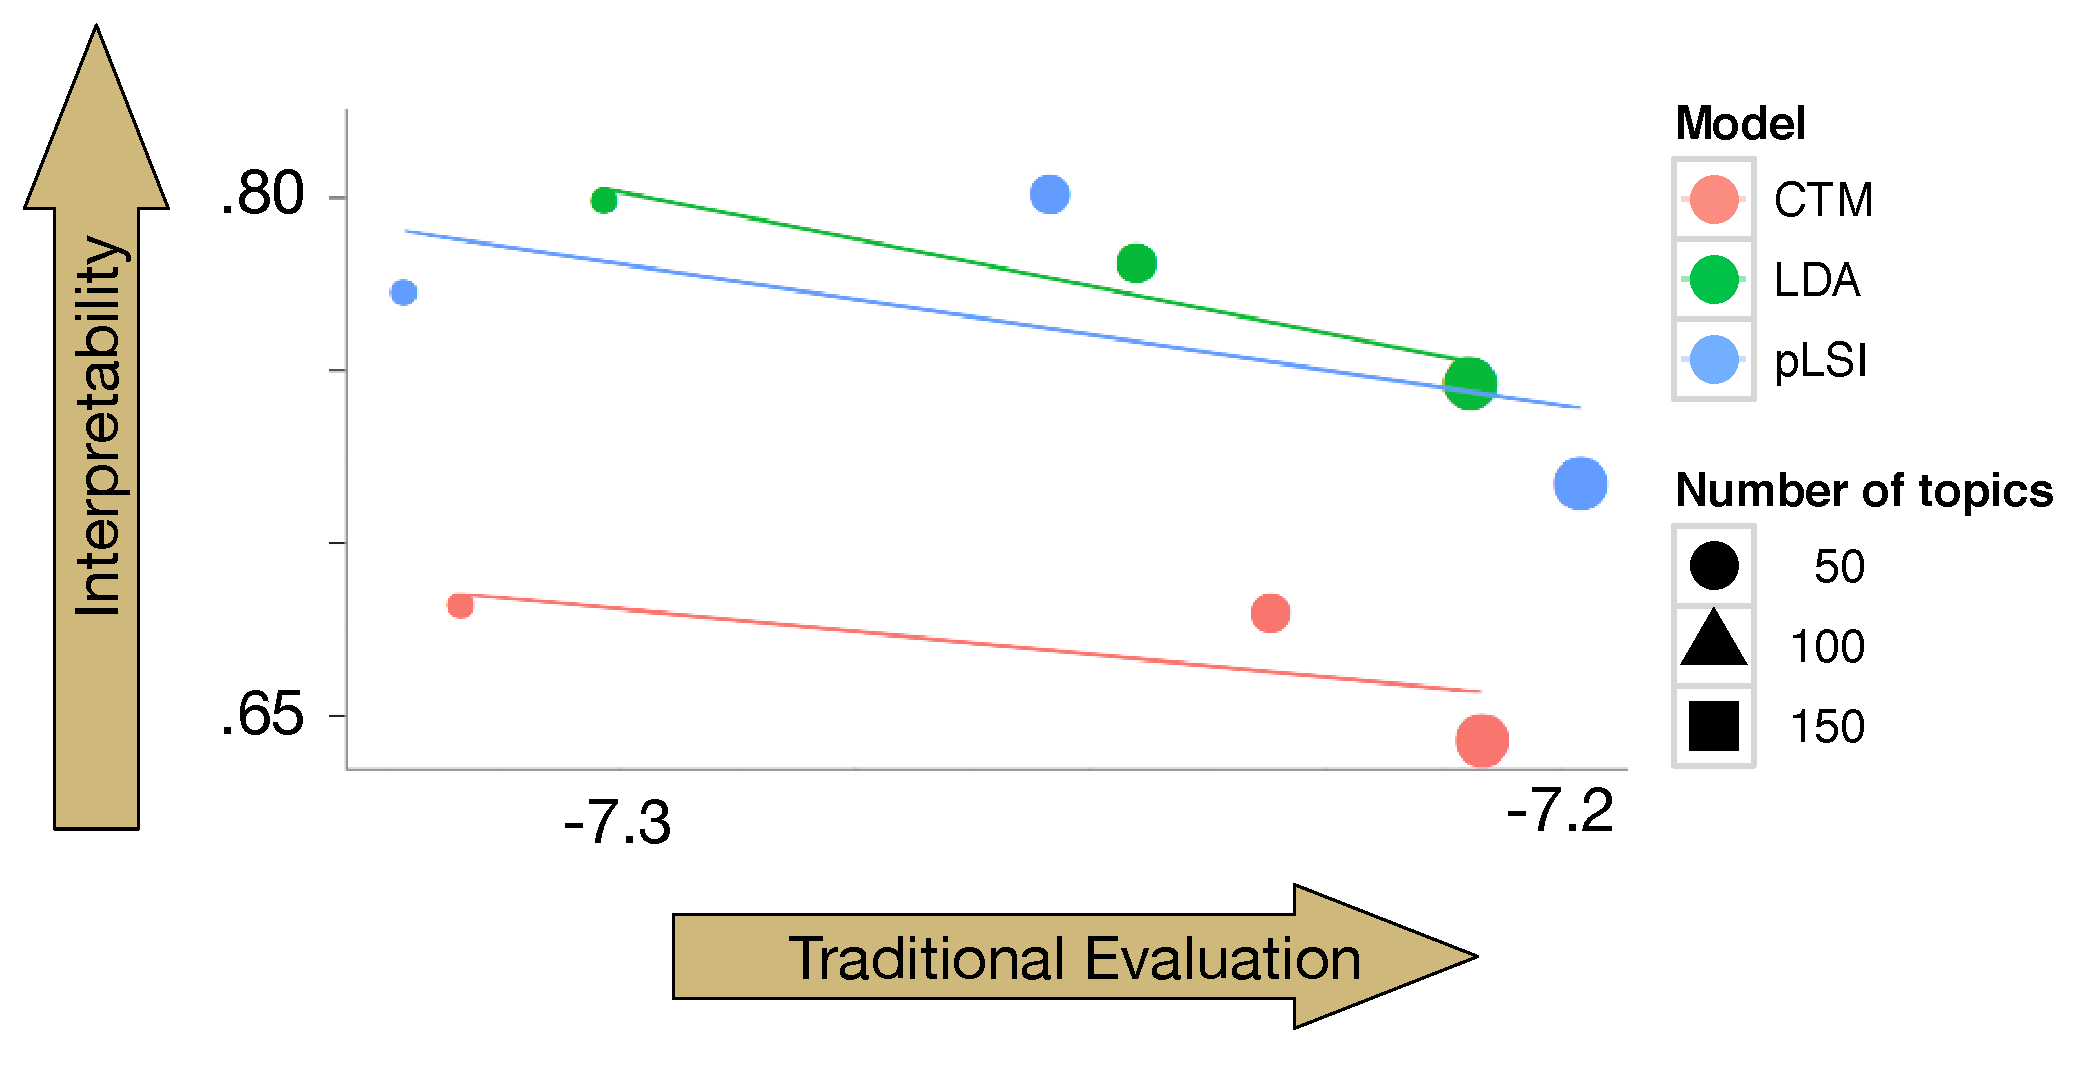
\includegraphics[width=.5\linewidth]{images/prec_ll_4}
\end{center}

Since this humbling discovery, I've built topic models that are a
collaboration between humans and computers.  The computer starts by
proposing an organization of the data.  The user separates confusing
clusters or joins similar clusters together~\cite{hu-14:itm}, an
improvement over the ``take it or leave it'' philosophy of most
machine learning algorithms.

Focusing on collaboration also requires algorithms that are low
latency (not just high throughput). We extended the
geometric interpretations of admixture models developed by Arora et
al.~\cite{arora-12} to multi-anchor topics~\cite{lund-17} and
multi-lingual topics~\cite{Yuan-18}.
%
These are much faster than traditional probabilistic topic
models---they can handle millions of documents in seconds---but they
are less well understood theoretically and less used in practice.
%
Thus, we also developed better understanding of the projections of
multilingual representations via graph theory~\cite{Fujinuma-19} and
the convergence of alternating projections~\cite{Zhang-19}.

After we proposed our ``reading tea leaves'' evaluation, it's
heartening that \newcite{lau}{14} and their ``machine reading tea
leaves'' (which correlate with our human measures) became a standard
topic model evaluation: in a survey of forty recent topic modeling
papers, {\bf all but four} use a form of their coherence evaluation.
%
However, as we argue in \newcite{hoyle}{21}, you cannot just use this
evaluation forever and forget about humans.
%
In that same survey, {\bf none} of those papers do a human evaluation.
%
As topic models evolve (e.g., incorporating
neural components), you need to validate that these automatic metrics
still correlate with whether it is useful for a human--computer
collaboration.

\section{Teaming as an Evaluation}

Within the \abr{hci} community, we have argued for the foundations of
what should go into human--computer collaborations: computers that incorporate
users' suggestions~\cite{kumar-19}; explanations with
accountability~\cite{smith-20}; and stable
explanations~\cite{smith-20:adherence}.

In addition to these human-centered understanding of users' needs and
desires, we've developed machine learning approaches to measure how
well users complete a task.
%
For example, for a question answering task, we measured how much the
accuracy of the human--computer \emph{team} increases with different
explanations and found that explanations help all users but that
novices are easily overwhelmed~\cite{feng-19}.
%
In follow-on work, we learned how to explicitly optimize explanations
for individual users~\cite{feng-22}.


\section{Connecting with Social Science: Pedagogy, Framing, and Deception}

The reverse of cooperation is human competition; it also has much to
teach computers.
%
I've increasingly looked at language-based games whose clear goals and
intrinsic fun speed research progress.
%
For example, in the board game \emph{Diplomacy}, users
chat with each other while marshaling armies for world conquest. Alliances are
fluid: friends are betrayed and enemies embraced as the game develops.
%
However,
users' conversations let us predict when friendships break.

Thus, we argued that Diplomacy would be an exciting testbed for
natural language processing, and our 2015 paper is---to the best of
our knowledge---the first \abr{nlp} research on Diplomacy.
%
Before a betrayal, betrayers write ostensibly friendly messages and become more polite, stop talking about the future, and change how \emph{much} they write~\cite{niculae-15}.
%
In follow-on work, we developed a dataset that predict both when users
lie to each other and when recipients of lies detect
deception~\cite{Peskov-20}.
%
Diplomacy may be a nerdy game, but it is a fruitful testbed to teach
computers to understand messy, emotional human interactions.
%
We are continuing to look into these questions with researchers from
across the nation in a new \abr{darpa} program: \abr{shade}, which
focuses on Diplomacy as a testbed for understanding deception.

Recently, the use of \abr{nlp} methods in the game of Diplomacy has
been the subject of highly-publicized papers by DeepMind in Nature
Communications~\cite{kramar-22} and Meta in Science~\cite{bakhtin-22}.
%
The Meta paper, like our 2020 paper, used a classifier to detect
deceptive statements.
%
The DeepMind paper built a game theoretic understanding of when
betrayal should happen, building on our descriptive investigation of
deception in human games.

A game with higher stakes is politics. However, just like Diplomacy,
the words that people use reveal their underlying goals; computational
methods can help expose the ``moves'' political players can use. With
collaborators in political science, we've built models that: show when
politicians in debates strategically change the topic to influence
others~\cite{nguyen-12,Nguyen-14b}; frame topics to reflect political
leanings~\cite{nguyen-13:shlda}; use subtle linguistic phrasing to
express their political leaning~\cite{iyyer-14a}; or create political
subgroups with larger political
movements~\cite{Nguyen:Boyd-Graber:Resnik:Miler-2015}.

Because political discourse is built on a common set of commonly
accepted facts, we have focused on developing fact checking: datasets
for general knowledge fact checking~\cite{eisenschlos-21} and climate
change fact checking~\cite{Diggelmann-20}.
%
However, because fact checking is part of an information arms race, we
need to build these examples as part of a human-in-the-loop
adversarial process, which I'm exploring in an ongoing collaboration
with journalism professor Naeemul Hassan that extends my question
answering work, which I talk about next.

\section{Human-in-the-Loop Adversarial Examples}

One of the most fun aspects of my research has been building
trivia-playing robots~\cite{boyd-graber-12,iyyer-14b,iyyer-15}; beyond research papers, our system has faced off against former Jeopardy
champions in front of hundreds high school
students\footnote{\url{https://www.youtube.com/watch?v=LqsUaprYMOw}}
and against researchers at NeurIPS 2015 (which won the best
demonstration award).
%
But after defeating some of the smartest trivia players, did I
actually believe that our system was better at question answering?
%
No!

Adversarial examples first came out of the vision community: add a
small epsilon to an example and suddenly a object detector calls a
turtle a gun~\cite{athalye-18}.\footnote{Point of personal pride: I
mentored Kevin on another research project~\cite{he-16}, but
I myself had nothing to do with this later adversarial work.}
%
While others have attempted to create adversarial examples for
language using paraphrasing, it's hard to know if the changes are
perceptually negligible (``who wrote the invisible man''---a question with the answer H.G. Wells---is
fundamentally different from ``who wrote the man you can't see''---an ill-formed questions---as is
``who wrote the book invisible man''---a question with the answer Ralph Ellison) and
it's hard to ``add epsilon'' to a discrete word.

Consistent with the theme of my research, my \abr{nsf career} grant
added a \emph{human in the loop} to generate novel adversarial
language examples that can provide new training examples to make
\abr{ai} more robust and to expose what \abr{ai} cannot (yet) do.
%
With Eric Wallace, an undergraduate student, we built a system that
could help an expert trivia question writer to stump a computer: as
the author writes the question, it shows the author what the system is
thinking~\cite{wallace-18}.
%
And it worked, even generalizing across models~\cite{wallace-19} (an
example written with an \abr{ir} model still stumps a neural model).
%
After we introduced human-in-the-loop adversarial example generation,
Meta/Facebook adopted this framework with gusto~\cite{bartolo-20} in
their Dynabench framework, the Dynamic Adversarial Data Collection
workshop and call for proposals (which I'm grateful is funding our
continuing research in this area).

\section{But wait, there's more!}

Many of our best-cited papers are ``traditional'' papers that do
better on some task:
%
\begin{itemize*}
\item We developed deep averaging networks~\cite[\abr{dan}]{iyyer-15}, a simple model still used in the 
transformer age~\cite{ye-22}.
\item In question answering, we proposed new evaluation mechanisms
  for knowing if an answer is correct~\cite{si-21} and improved
  information retrieval to answer complicated
  questions~\cite{elgohary-19,zhao-20,shi-20}.

\item We also introduced reinforcement learning to \emph{simultaneous
machine interpretation}~\cite{Grissom:He:Boyd-Graber:Morgan-2014}, a
  language-based task that requires significant human intuition,
  insight, and---for those who want to become
  interpreters---training.\footnote{This framework---using
  reinforcement learning to capture human strategies---was featured in
  Liang Huang's \abr{acl} keynote.} We learned tricks from
  professional human interpreters---passivizing sentences and guessing
  the verb---to translate sentences sooner~\cite{He-15}, letting
  speakers and algorithms cooperate together and enabling more natural
  cross-cultural communication.  We also use reinforcement
  learning to learn machine translation feedback from noisy
  supervision such as star ratings on a webpage~\cite{nguyen-17}.
\end{itemize*}

This work doesn't \emph{yet} fit nicely into the human--computer
collaboration narrative, but these more complex tasks are part of my
broader vision for where my research will go: state-of-the-art models
built to support human decisions, not replace them.  And that requires
the low-latency models built to react to input ``like a human''
described above.

\section{Future Work}

I hope that I've convinced you that to get more effective \abr{ai}, we
need to measure how well it works (and plays) \emph{with} humans.
%
This is a problem that requires solutions in the form of new data, algorithms, and evalutions, and I
hope to advance in all three areas.

{\bf Data.}
%
Existing datasets are not diverse and do
not reflect the kinds of interactions people from diverse backgrounds
have with \abr{ai} systems.
%
In question answering, Google's Natural Questions, SQuAD, and other
datasets contain entities that are overwhelmingly male and either
American on British~\cite{gor-21}.
%
In newly funded \abr{nih} research, we're working with answering
questions specifically in complicated, code-switched environments with
less educated users trying to navigate the healthcare landscape.
%
These linguistically, acoustically, and socio-economically diverse
samples will help provide more realistic data for question answering
applications, replete with false presuppositions, ambiguity, and
shifting information needs.
%
We are also working with \abr{nist} to develop datasets that better
reflect a specific \emph{cultural} context: detecting when questions
are answered differently in Ghana than in the \abr{us} or topics that
only people in Bhutan care about (and would be neglected by
\abr{us}-centric datasets).

{\bf Algorithms.} In research recently funded by Meta, we're capitalizing on
the realization that the best way to get good datasets that reflect
the strengths and weaknesses of current \abr{ai} is to have users in the loop to generate adversarial data.
%
While our previous adversarial datasets focused on a single
system---find a question \emph{this} neural system cannot answer---we
are expanding our search to \emph{learn} how to help users best
engineer adversarial examples, a natural extension of our work using
bandit algorithms to improve explanations.
%
While our goal in that work was to get the human--computer team to
answer a question correctly, we flip the script to create explanations
that help the user craft examples the computer cannot answer.

However, those algorithms are for \emph{supervised} tasks where there
is a known answer.
%
For \emph{unsupervised} tasks like understanding the themes in a
document collection, we need algorithms
that are not just transparent but that are \emph{fast}: the primary
goal is exploration of the dataset, and the user needs to be able to
quickly provide feedback to the algorithm.
%
The algorithm then needs to update quickly given that feedback.

To develop more robust algorithms, we are building training approaches
that---as a conversation develops---explicitly build representations that
capture the theory of mind of conversation participants and the
current ``question under discussion''.
%
We plan to apply this both in our Diplomacy game that captures
strategic negotiations (detecting when a negotiation partner is
angling for a particular resolution implicitly or when they are
negotiation in bad faith) and in the information seeking question
answering context (where a question can be posed imperfectly,
revealing a false assumption or a lack of background information).
%
% By reverse engineering the causal mechanism of why a particual theme
% or topic was broached in an interaction, the \abr{ai} interlocutor can
% better frame their reply, probing underlying assumptions or
% developing an effective ``counter''.

While eventually we will need to connect to expensive, difficult to
compute neural models, many user updates can be approximated by fast
spectral or probabilistic algorithms.
%
We will design fast, browser-based Javascript approximations of these
complicated neural models, to allow users to quickly interact with the
models, get a result, and continue before reconciling the solution later.
%
% However, because these approximations are only approximations, we need
% to reconcile the approximate solution with the ``gold standard'' model
% on a \abr{gpu}-powered server.

{\bf Evaluation.}
%
Where computers have strengths that go beyond what a human can do, we
need to know if it would be wise to build evaluations that can we
will build interactive systems that help users come to a correct
answer through a process they trust, measure that process, and
optimize to encourage this cooperation.
%
This requires basic engineering---ensuring all of the components of
a system are efficient and low latency---and user modeling, as we
cannot assume that every user will have the same knowledge and
capabilities.
%
% The next step requires careful vetting in diverse domains to validate
% that users' skills and knowledge are actually augmented by the help of
% the computer.
%
% We aim to focus on multiple areas: question answering in a single
% language~\cite{He-22}, question answering across
% languages~\cite{han-22}, and the strategic game of Diplomacy.

As these systems become more capable and usable, we can no longer
assume that our model of the user should remain static: the user will
learn and adapt to the system.
%
This makes modeling more complicated, but it also allows for employing
these models in educational settings through examples ordered in a
curriculum: expanding the frontier of what the user knows, reinforcing
weaker knowledge, and using strategies to both educate and explain
information from the \abr{ai}.
%
% This will require matching users' capabilities with what models can
% offer.

But interactions with individual people are not how \abr{ai} will be a
part of 21\textsuperscript{st} society: it will be interactions with
\emph{populations}.
%
Thus, we need to have models and systems that capture population-level
interactions.
%
Helping detect misinformation online, working collaboratively with
authors to craft effective counter-measures, and to propagate that
within a social network.
%
This builds on our fake news systems and our deception detection work,
but will also require deeper collaboration with social scientists and
journalists to develop the interfaces and the models to build
human--computer \abr{ai} that informs and helps society as a whole.


%% \vspace{12cm}

%%  \parbox{\linewidth}{I certify that this
%%   statement is a current and accurate statement of my
%%   professional record to the best of my
%%   knowledge \flushright  
\includegraphics[width=.2\linewidth]{resume_src/signature} \\
%% \flushright  (\today{})}

\clearpage

%%%%%%%%%%%%%%%%%%%%%%%%%%%%%%%%

